\subsection{Software Design DAL Design}
På \autoref{fig:DAL-Klasse-7-17-18} herunder ses klassediagrammet over backend DAL, som benyttes til database access. 
Som det kan ses på diagrammet, indeholder DAL en database context, som benyttes til at forbinde backend applicationen til databasen. 
Derudover består DAL af fire overordnede funktioner, hvoraf de 3 tilhører en user story. 
Den sidste funktion benyttes når vi starter spillet, til at lave rumbeskrivelser.\\

\begin{figure}[H]
\centering
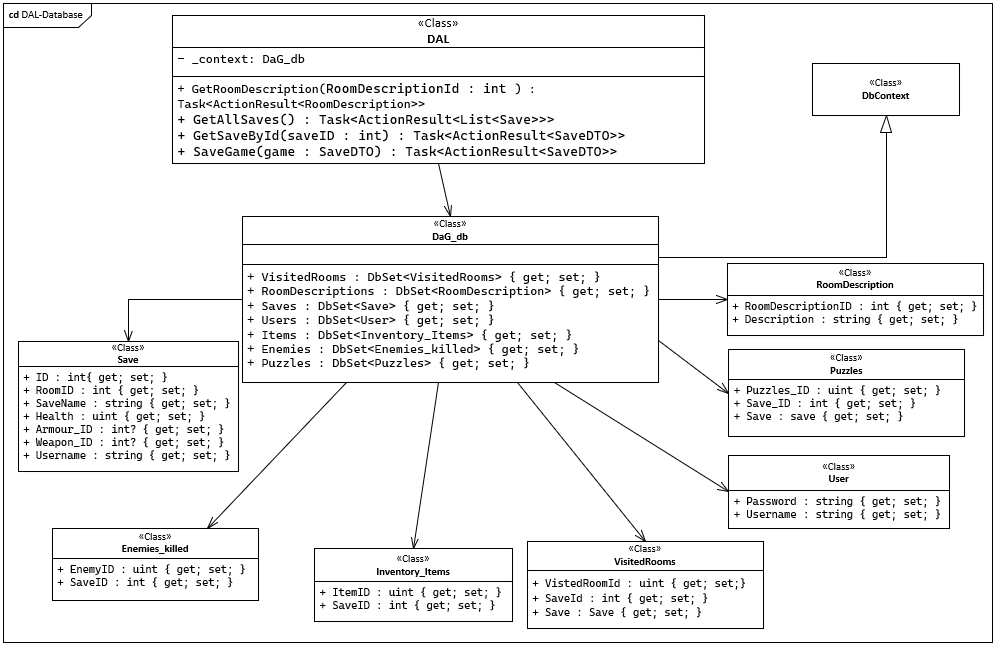
\includegraphics[width = \textwidth]{02-Body/Images/DAL-Database/DAL-DB-CD.PNG}
\caption{Samlet klasse diagram for User story 8, 15, 17 og 18 med DAL db context og entitetsklasser.
For læseligheden er DAL klassen ikke forbundet til forskellige entitetsklasser selvom disse benyttes.}
\label{fig:DAL-Klasse-7-17-18}
\end{figure}

Følgende funktion som beskrives på \autoref{fig:DAL-Sekvens-RumBeskrivelser} benyttes når spil klienten startes, da beskrivelser af rum ikke ændre sig gennem spillets levetid, i den nuværende itteration.\\

\begin{figure}[H]
\centering
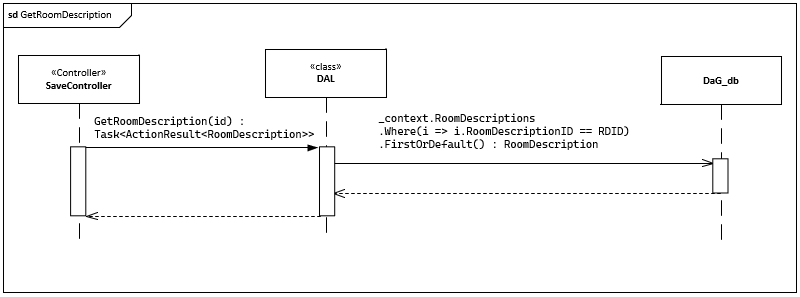
\includegraphics[width = \textwidth]{02-Body/Images/DAL-Database/RoomDescriptionSd.PNG}
\caption{Sekvensdiagram om læsning af en rumbeskrivelse}
\label{fig:DAL-Sekvens-RumBeskrivelser}
\end{figure}

Navn: GetRoomDescription \\
Parametre: int RoomDescriptionId \\
Returtype: Task\l ActionResult\l RoomDescription\g\g\\
Beskrivelse: Denne funktion finder og returnerer en beskrivelse for det valgte RoomDescriptionID. 
Dette kan også ses på sekvensdiagrammet på figur \autoref{fig:DAL-Sekvens-RumBeskrivelser}.


\subsubsection{User story funktioner}
De følgende 3 funktioner benyttes til udførelse af forskellige user stories.
Det drejer sig om:
\begin{itemize}
\item User story 15 – Save game
\item User story 8 - Save - No Combat  + User story 17 – Load game list 
\item User story 18 – Load game \\
\end{itemize}

Funktionen GetById benyttes til at udfører user story 18.
Her skal der loades et gemt spil, som brugeren nu ønsker at spille. 
Dette kan også ses på sekvensdiagrammet på \autoref{fig:DAL-Sekvens-18}.\\

\begin{figure}[H]
\centering
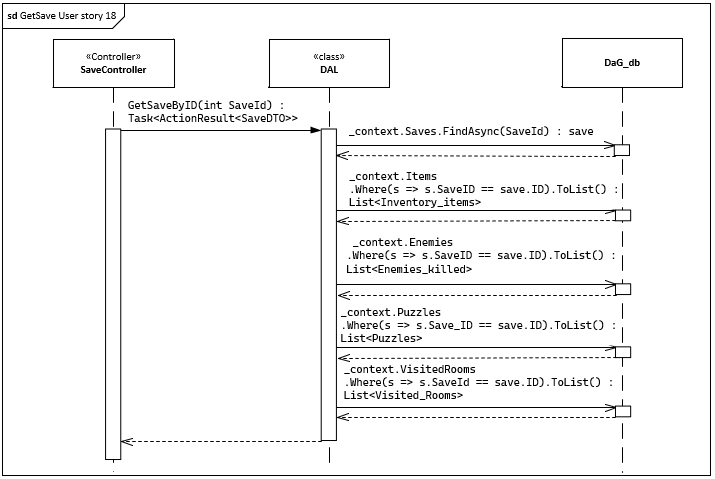
\includegraphics[width = \textwidth]{02-Body/Images/DAL-Database/GetSavesByIdSd.PNG}
\caption{Sekvensdiagram for user story 18 GetSaveById som beskriver queries til databasen for at hente et specifikt save og dens tilhørende information}
\label{fig:DAL-Sekvens-18}
\end{figure}

Funktionsbeskrivelse:\\
Navn: GetSaveById \\
Parametre: int saveID\\
Returtype: Task\l ActionResult\l SaveDTO\g\g\\
Beskrivelse: Denne funktion finder det save med det medsendte ID, samt tilhørende lister, indsætter værdier i et SaveDTO objekt, hvorefter det returneres.\\

Funktionsbeskrivelser og sekvensdiagrammer for de 2 andre user story funktioner kan findes \textbf{REF TIL TEKNISK BILAG}